\PassOptionsToPackage{unicode=true}{hyperref} % options for packages loaded elsewhere
\PassOptionsToPackage{hyphens}{url}
%
\documentclass[
  ignorenonframetext,
]{beamer}
\usepackage{pgfpages}
\setbeamertemplate{caption}[numbered]
\setbeamertemplate{caption label separator}{: }
\setbeamercolor{caption name}{fg=normal text.fg}
\beamertemplatenavigationsymbolsempty
% Prevent slide breaks in the middle of a paragraph:
\widowpenalties 1 10000
\raggedbottom
\setbeamertemplate{part page}{
  \centering
  \begin{beamercolorbox}[sep=16pt,center]{part title}
    \usebeamerfont{part title}\insertpart\par
  \end{beamercolorbox}
}
\setbeamertemplate{section page}{
  \centering
  \begin{beamercolorbox}[sep=12pt,center]{part title}
    \usebeamerfont{section title}\insertsection\par
  \end{beamercolorbox}
}
\setbeamertemplate{subsection page}{
  \centering
  \begin{beamercolorbox}[sep=8pt,center]{part title}
    \usebeamerfont{subsection title}\insertsubsection\par
  \end{beamercolorbox}
}
\AtBeginPart{
  \frame{\partpage}
}
\AtBeginSection{
  \ifbibliography
  \else
    \frame{\sectionpage}
  \fi
}
\AtBeginSubsection{
  \frame{\subsectionpage}
}
\usepackage{lmodern}
\usepackage{amssymb,amsmath}
\usepackage{ifxetex,ifluatex}
\ifnum 0\ifxetex 1\fi\ifluatex 1\fi=0 % if pdftex
  \usepackage[T1]{fontenc}
  \usepackage[utf8]{inputenc}
  \usepackage{textcomp} % provides euro and other symbols
\else % if luatex or xelatex
  \usepackage{unicode-math}
  \defaultfontfeatures{Scale=MatchLowercase}
  \defaultfontfeatures[\rmfamily]{Ligatures=TeX,Scale=1}
\fi
\usetheme[]{Darmstadt}
\usecolortheme{rose}
\usefonttheme{structurebold}
% use upquote if available, for straight quotes in verbatim environments
\IfFileExists{upquote.sty}{\usepackage{upquote}}{}
\IfFileExists{microtype.sty}{% use microtype if available
  \usepackage[]{microtype}
  \UseMicrotypeSet[protrusion]{basicmath} % disable protrusion for tt fonts
}{}
\makeatletter
\@ifundefined{KOMAClassName}{% if non-KOMA class
  \IfFileExists{parskip.sty}{%
    \usepackage{parskip}
  }{% else
    \setlength{\parindent}{0pt}
    \setlength{\parskip}{6pt plus 2pt minus 1pt}}
}{% if KOMA class
  \KOMAoptions{parskip=half}}
\makeatother
\usepackage{xcolor}
\IfFileExists{xurl.sty}{\usepackage{xurl}}{} % add URL line breaks if available
\IfFileExists{bookmark.sty}{\usepackage{bookmark}}{\usepackage{hyperref}}
\hypersetup{
  pdftitle={Intro Datenanalyse mit R - Warum R eine gute Wahl ist?},
  pdfauthor={Jan-Philipp Kolb},
  pdfborder={0 0 0},
  breaklinks=true}
\urlstyle{same}  % don't use monospace font for urls
\newif\ifbibliography
\usepackage{graphicx,grffile}
\makeatletter
\def\maxwidth{\ifdim\Gin@nat@width>\linewidth\linewidth\else\Gin@nat@width\fi}
\def\maxheight{\ifdim\Gin@nat@height>\textheight\textheight\else\Gin@nat@height\fi}
\makeatother
% Scale images if necessary, so that they will not overflow the page
% margins by default, and it is still possible to overwrite the defaults
% using explicit options in \includegraphics[width, height, ...]{}
\setkeys{Gin}{width=\maxwidth,height=\maxheight,keepaspectratio}
\setlength{\emergencystretch}{3em}  % prevent overfull lines
\providecommand{\tightlist}{%
  \setlength{\itemsep}{0pt}\setlength{\parskip}{0pt}}
\setcounter{secnumdepth}{-2}

% set default figure placement to htbp
\makeatletter
\def\fps@figure{htbp}
\makeatother


\title{Intro Datenanalyse mit R - Warum R eine gute Wahl ist?}
\author{Jan-Philipp Kolb}
\date{06 Mai, 2019}

\begin{document}
\frame{\titlepage}

\begin{frame}{Um rein zu kommen}
\protect\hypertarget{um-rein-zu-kommen}{}

\begin{block}{Kleine Vorstellungsrunde}

\begin{itemize}
\tightlist
\item
  Wo kommt Ihr her?
\item
  Wo arbeitet und studiert Ihr?
\item
  Habt Ihr Erfahrungen mit Programmiersprachen / Statistiksoftware? Wenn
  ja welche?
\item
  Was sind Eure Erwartungen für diesen Kurs?
\end{itemize}

\end{block}

\end{frame}

\begin{frame}{Disclaimer/ Informationen vorab}
\protect\hypertarget{disclaimer-informationen-vorab}{}

Normalerweise gibt es große Unterschiede bei Vorkenntnissen und
Fähigkeiten - bitte gebt Bescheid, wenn es zu schnell oder zu langsam
geht oder etwas unklar geblieben ist.

\begin{itemize}
\tightlist
\item
  Wenn es Fragen gibt - immer fragen
\item
  In diesem Kurs gibt es viele
  \href{http://web.math.ku.dk/~helle/R-intro/exercises.pdf}{\textbf{Übungen}},
  denn das Programmieren / die Nutzung von R lernt man am Ende nur
  allein.
\item
  Ich habe viele \href{https://www.showmeshiny.com/}{\textbf{Beispiele}}
  - probiert sie aus
\item
  R macht mehr Spaß zusammen - arbeitet zusammen!
\end{itemize}

\end{frame}

\begin{frame}{Erwartungen und Anforderungen}
\protect\hypertarget{erwartungen-und-anforderungen}{}

\begin{block}{Das kann diese Schulung vermitteln:}

\begin{itemize}
\tightlist
\item
  Eine praxisnahe Einführung in die statistische Programmiersprache R
\item
  Erlernen einer Programmier-Strategie
\item
  Guten Stil
\item
  Die Vorzüge graphischer Datenanalyse
\end{itemize}

\end{block}

\begin{block}{Das kann sie nicht leisten:}

\begin{itemize}
\tightlist
\item
  Eine Einführungsveranstaltung in die Statistik geben
\item
  Grundlegende datenanalytische Konzepte vermitteln
\item
  Verständnis zementieren
\item
  Das Trainieren abnehmen
\end{itemize}

\end{block}

\end{frame}

\begin{frame}{Gründe R zu nutzen\ldots{}}
\protect\hypertarget{grunde-r-zu-nutzen}{}

\begin{itemize}
\item
  \ldots{} R ist eine
  \href{https://stackoverflow.com/questions/1546583/what-is-the-definition-of-an-open-source-programming-language}{\textbf{quelloffene
  Sprache}}
\item
  \ldots{} hervorragende
  \href{http://matthewlincoln.net/2014/12/20/adjacency-matrix-plots-with-r-and-ggplot2.html}{\textbf{Grafiken}},
  \href{https://www.r-bloggers.com/3d-plots-with-ggplot2-and-plotly\%20/}{\textbf{Grafiken}},
  \href{https://procomun.wordpress.com/2011/03/18/splomr/}{\textbf{Grafiken}}
\item
  \ldots{} \href{https://github.com/Japhilko/RInterfaces}{\textbf{R kann
  in Kombination mit anderen Programmen verwendet werden}} - z.B. zur
  \href{https://github.com/Japhilko/RInterfaces/blob/master/slides/Datenimport.md}{\textbf{Verknüpfung
  von Daten}}
\item
  \ldots{} R kann
  \href{https://cran.r-project.org/web/packages/MplusAutomation/index.html}{\textbf{zur
  Automatisierung}} verwendet werden
\item
  \ldots{} Breite und aktive Community -
  \href{https://www.r-bloggers.com/}{\textbf{Man kann die Intelligenz
  anderer Leute nutzen ;-)}}
\end{itemize}

\end{frame}

\begin{frame}{Gründe}
\protect\hypertarget{grunde}{}

\begin{itemize}
\tightlist
\item
  R ist \href{http://www.inside-r.org/why-use-r}{frei verfügbar}. Es
  kann umsonst \href{http://mirrors.softliste.de/cran/}{runtergeladen}
  werden.
\item
  R ist eine
  \href{https://de.wikipedia.org/wiki/Skriptsprache}{Skriptsprache}
\item
  Gute Möglichkeiten für die
  \href{http://research.stowers-institute.org/efg/R/}{Visualisierung}
  (\href{http://www.sr.bham.ac.uk/~ajrs/R/r-gallery.html}{Link} )
\item
  R wird immer
  \href{https://twitter.com/josiahjdavis/status/559778930476220418}{populärer}
\item
  \href{http://blog.revolutionanalytics.com/popularity/}{Popularität von
  R}
\end{itemize}

\end{frame}

\begin{frame}{R kann in Kombination mit anderen Programmen genutzt
werden\ldots{}}
\protect\hypertarget{r-kann-in-kombination-mit-anderen-programmen-genutzt-werden}{}

\begin{figure}
\centering
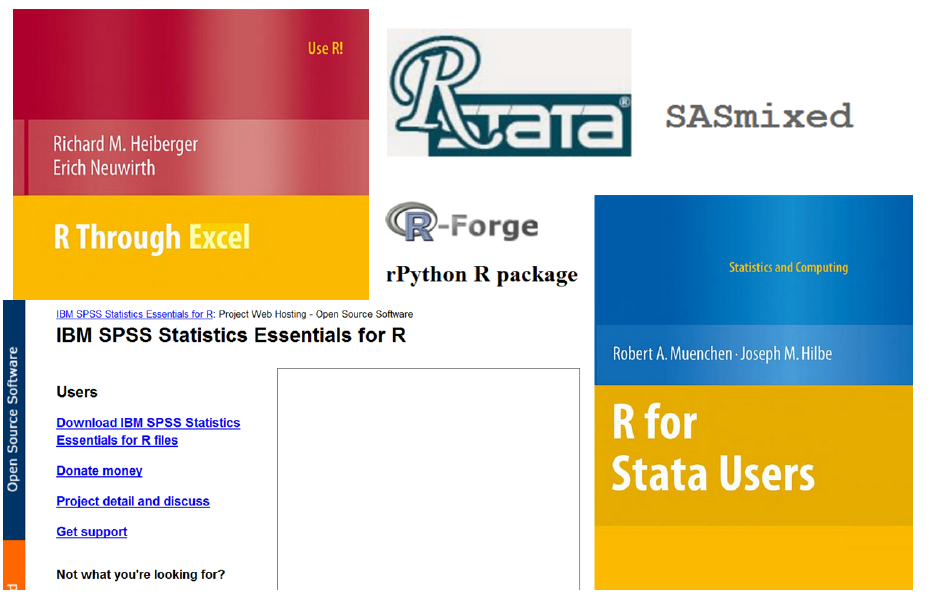
\includegraphics{figure/Rinterfaces.PNG}
\caption{Schnittstellen zu R**}
\end{figure}

\begin{itemize}
\tightlist
\item
  Schnittstelle zu:
  \href{https://cran.r-project.org/web/packages/reticulate/vignettes/calling_python.html}{\textbf{Python}},
  \href{https://www.springer.com/de/book/9781441900517}{\textbf{Excel}},
  \href{https://www.ibm.com/support/knowledgecenter/en/SSFUEU_7.2.0/com.ibm.swg.ba.cognos.op_capmod_ig.7.2.0.doc/t_essentials_for_r_statistics.html}{\textbf{SPSS}},
  \href{https://cran.r-project.org/web/packages/SASmixed/index.html}{\textbf{SAS}},
  \href{https://cran.r-project.org/web/packages/RStata/index.html}{\textbf{Stata}}
\end{itemize}

\end{frame}

\begin{frame}{\href{https://gallery.shinyapps.io/cran-gauge/}{Die
Popularität von R}}
\protect\hypertarget{die-popularitat-von-r}{}

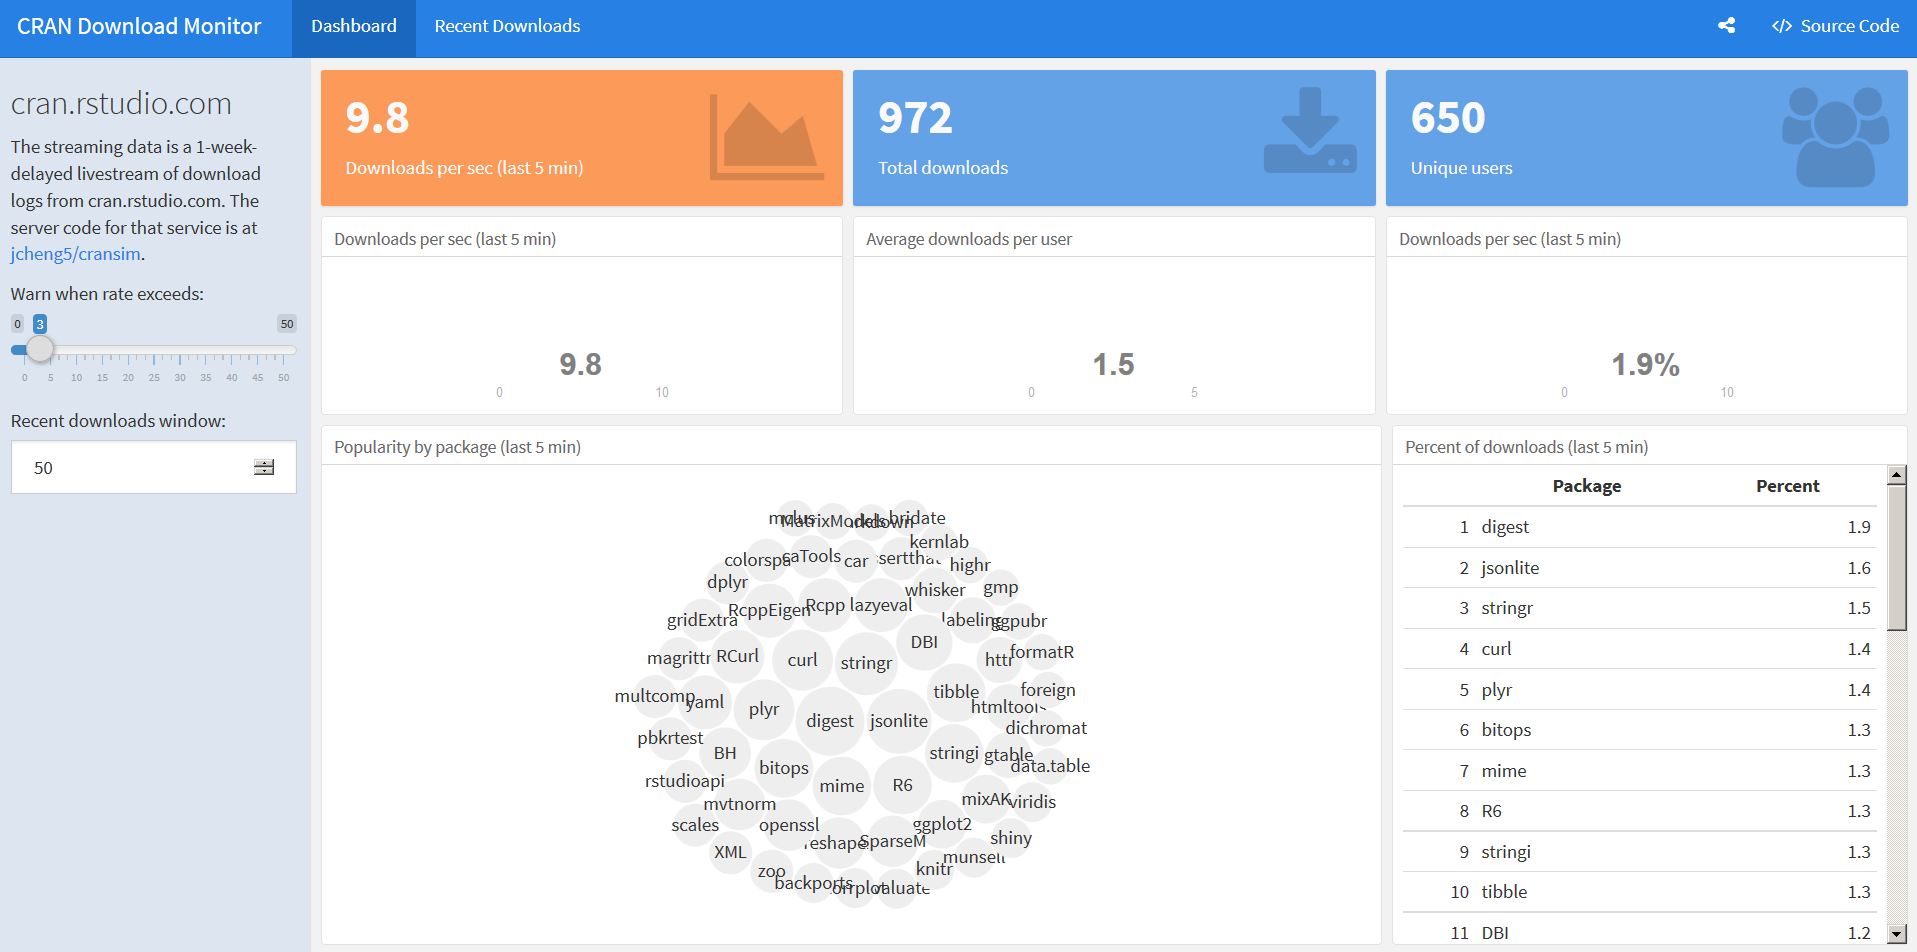
\includegraphics{figure/CRANdownloads.PNG}

\end{frame}

\begin{frame}{\href{https://www.bloomberg.com/news/articles/2013-04-18/faq-reinhart-rogoff-and-the-excel-error-that-changed-history}{R
sollte genutzt werden, weil andere Programme Fehler provozieren:}}
\protect\hypertarget{r-sollte-genutzt-werden-weil-andere-programme-fehler-provozieren}{}

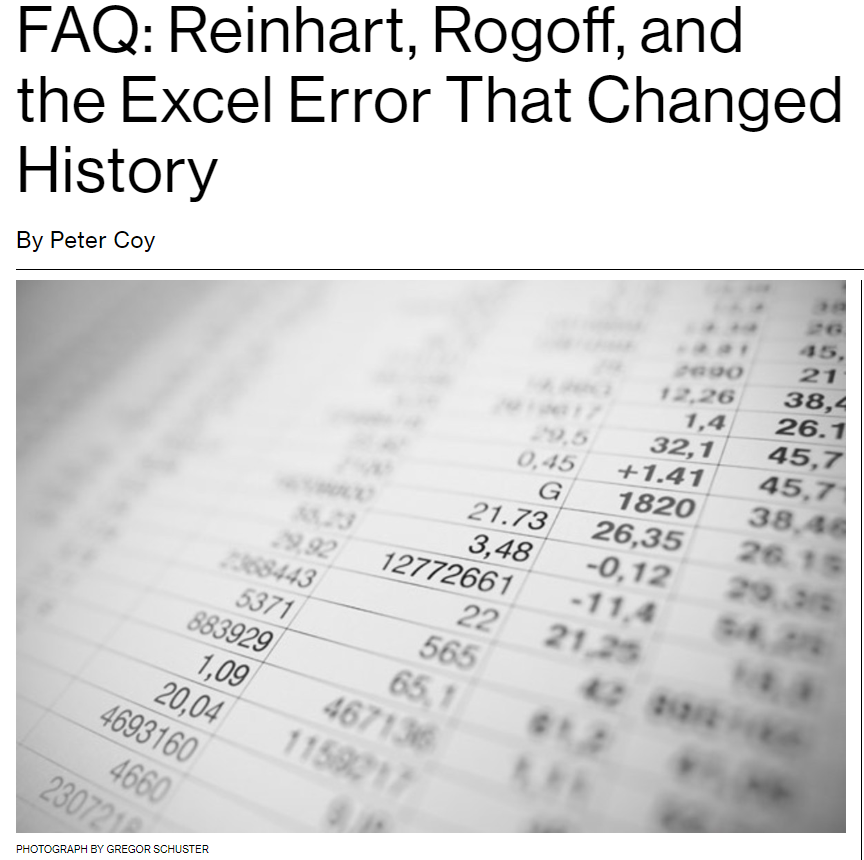
\includegraphics{figure/RheinhartRogoff.PNG}

\end{frame}

\begin{frame}{R herunterladen:}
\protect\hypertarget{r-herunterladen}{}

\url{http://www.r-project.org/}

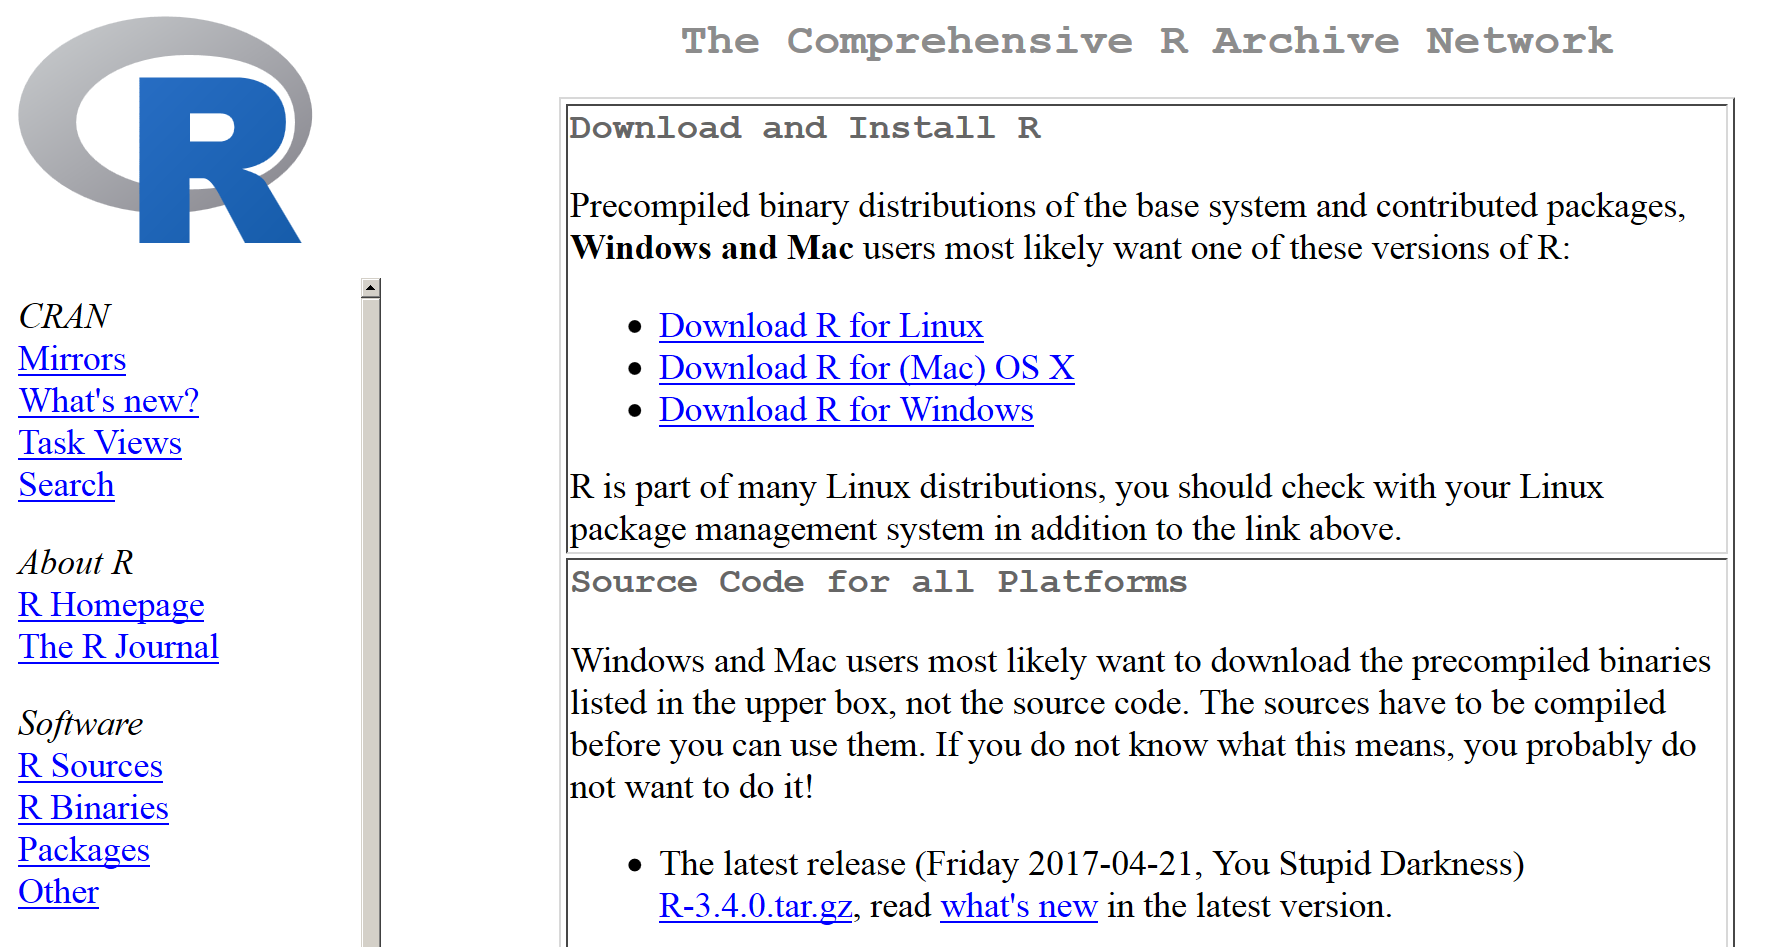
\includegraphics{figure/CRAN1picture.PNG}

\end{frame}

\begin{frame}{Links}
\protect\hypertarget{links}{}

\begin{itemize}
\item
  \href{http://www.r-bloggers.com/why-you-should-learn-r-first-for-data-science/}{Warum
  man R für Data Science lernen sollte}
\item
  \href{http://www.r-bloggers.com/rstudio-infoworld-2015-technology-of-the-year-award-recipient/}{R
  Technologie des Jahres}
\item
  \href{http://www.fastcolabs.com/3030063/why-the-r-programming-language-is-good-for-business}{Why
  R is Good for Business}
\item
  \href{http://www.r-bloggers.com/why-use-r/}{Warum R auf r-bloggers}
\item
  \href{http://www.ats.ucla.edu/stat/r/seminars/intro.htm}{Intro R}
\item
  \href{http://www.ats.ucla.edu/stat/r/sk/}{Intro R II}
\item
  \href{http://www.dataschool.io/python-or-r-for-data-science/}{Vergleich
  python und R}
\end{itemize}

\end{frame}

\begin{frame}{Probleme mit Excel}
\protect\hypertarget{probleme-mit-excel}{}

Weil andere Programme große Fehler haben:

\begin{itemize}
\item
  \href{http://blog.revolutionanalytics.com/2013/02/did-an-excel-error-bring-down-the-london-whale.html}{Excel
  bug}
\item
  \href{https://coffeehouse.dataone.org/2014/04/09/abandon-all-hope-ye-who-enter-dates-in-excel/}{Datum
  in Excel}
\end{itemize}


\includegraphics{figure/Abandon.PNG}

\end{frame}

\begin{frame}{\href{http://www.biomedcentral.com/1471-2105/5/80}{Probleme
mit Excel}}
\protect\hypertarget{probleme-mit-excel-1}{}


\includegraphics{figure/ExcelProblems.PNG}

\end{frame}

\begin{frame}{\href{https://www.inwt-statistics.de/blog-artikel-lesen/Statistik-Software-R_SAS_SPSS_STATA_im_Vergleich.html}{Vergleich
mit anderen Programmen}}
\protect\hypertarget{vergleich-mit-anderen-programmen}{}


\includegraphics{figure/SoftwareVergleich.PNG}

\end{frame}

\end{document}
